%%\documentclass[12pt,preprint]{aastex}

%% manuscript produces a one-column, double-spaced document:

%\documentclass[manuscript]{aastex}

%% preprint2 produces a double-column, single-spaced document:

 \documentclass[preprint2]{aastex}

%% \documentclass[preprint2,longabstract]{aastex}

\newcommand{\vdag}{(v)^\dagger}
\newcommand{\myemail}{jbyrne@ifa.hawaii.edu}


% ADDING THESE: -JPB
\usepackage{natbib}
\usepackage{amssymb,amsmath}

\shorttitle{3D CMEs Observed with STEREO}
\shortauthors{Byrne et al.}


\begin{document}

\title{Investigating the Robustness of the CORIMP CME Catalog Against Other Automated Catalogs and Manual Case Studies} %Statistical study of the events in the CORIMP Coronal Mass Ejection catalog from LASCO observations during the years 2000 to 2014}

\author{J. P. Byrne$^{1,2}$ et al}%, H. Morgan$^{3,4}$,  P. T. Gallagher$^{5}$, S. R. Habbal$^{2}$}
\affil{$^{1}$Rutherford Appleton Laboratory, STFC: RAL Space, Harwell Oxford, OX11 0QX, UK.\\
	$^{2}$Institute for Astronomy, University of Hawai'i, 2680 Woodlawn Drive, Honolulu, HI 96822, USA.\\
	%$^{3}$Sefydliad Mathemateg a Ffiseg, Prifysgol Aberystwyth, Ceredigion, Cymru, SY23 3BZ, UK.\\
	%$^{4}$Coleg Cymraeg Cenedlaethol, Y Llwyfan, Ffordd y Coleg, Caerfyrddin, Cymru, SA31 3EQ, UK.\\
	%$^{5}$School of Physics, Trinity College Dublin, College Green, Dublin 2, Ireland.
	%$^{5}$Trinity Centre for High Performance Computing, Trinity College Dublin, College Green, Dublin 2, Ireland.
	}


\begin{abstract}

CMEs are long known to be significant drivers of adverse space weather at Earth, but the physics governing their propagation is not fully understood. 

\end{abstract}

\keywords{Sun: coronal mass ejections (CMEs) --- Methods: miscellaneous --- Techniques: image processing}


\section{Introduction}


\section{Events}


\begin{figure*}[]
\centerline{\includegraphics[width=\linewidth]{images/20000418_four.pdf}}
\caption{.}
\label{}
\end{figure*}

\begin{figure*}[]
\centerline{\includegraphics[width=\linewidth]{images/20000418_corimp_kins1.pdf}}
\caption{.}
\label{}
\end{figure*}


\begin{figure}[]
\centerline{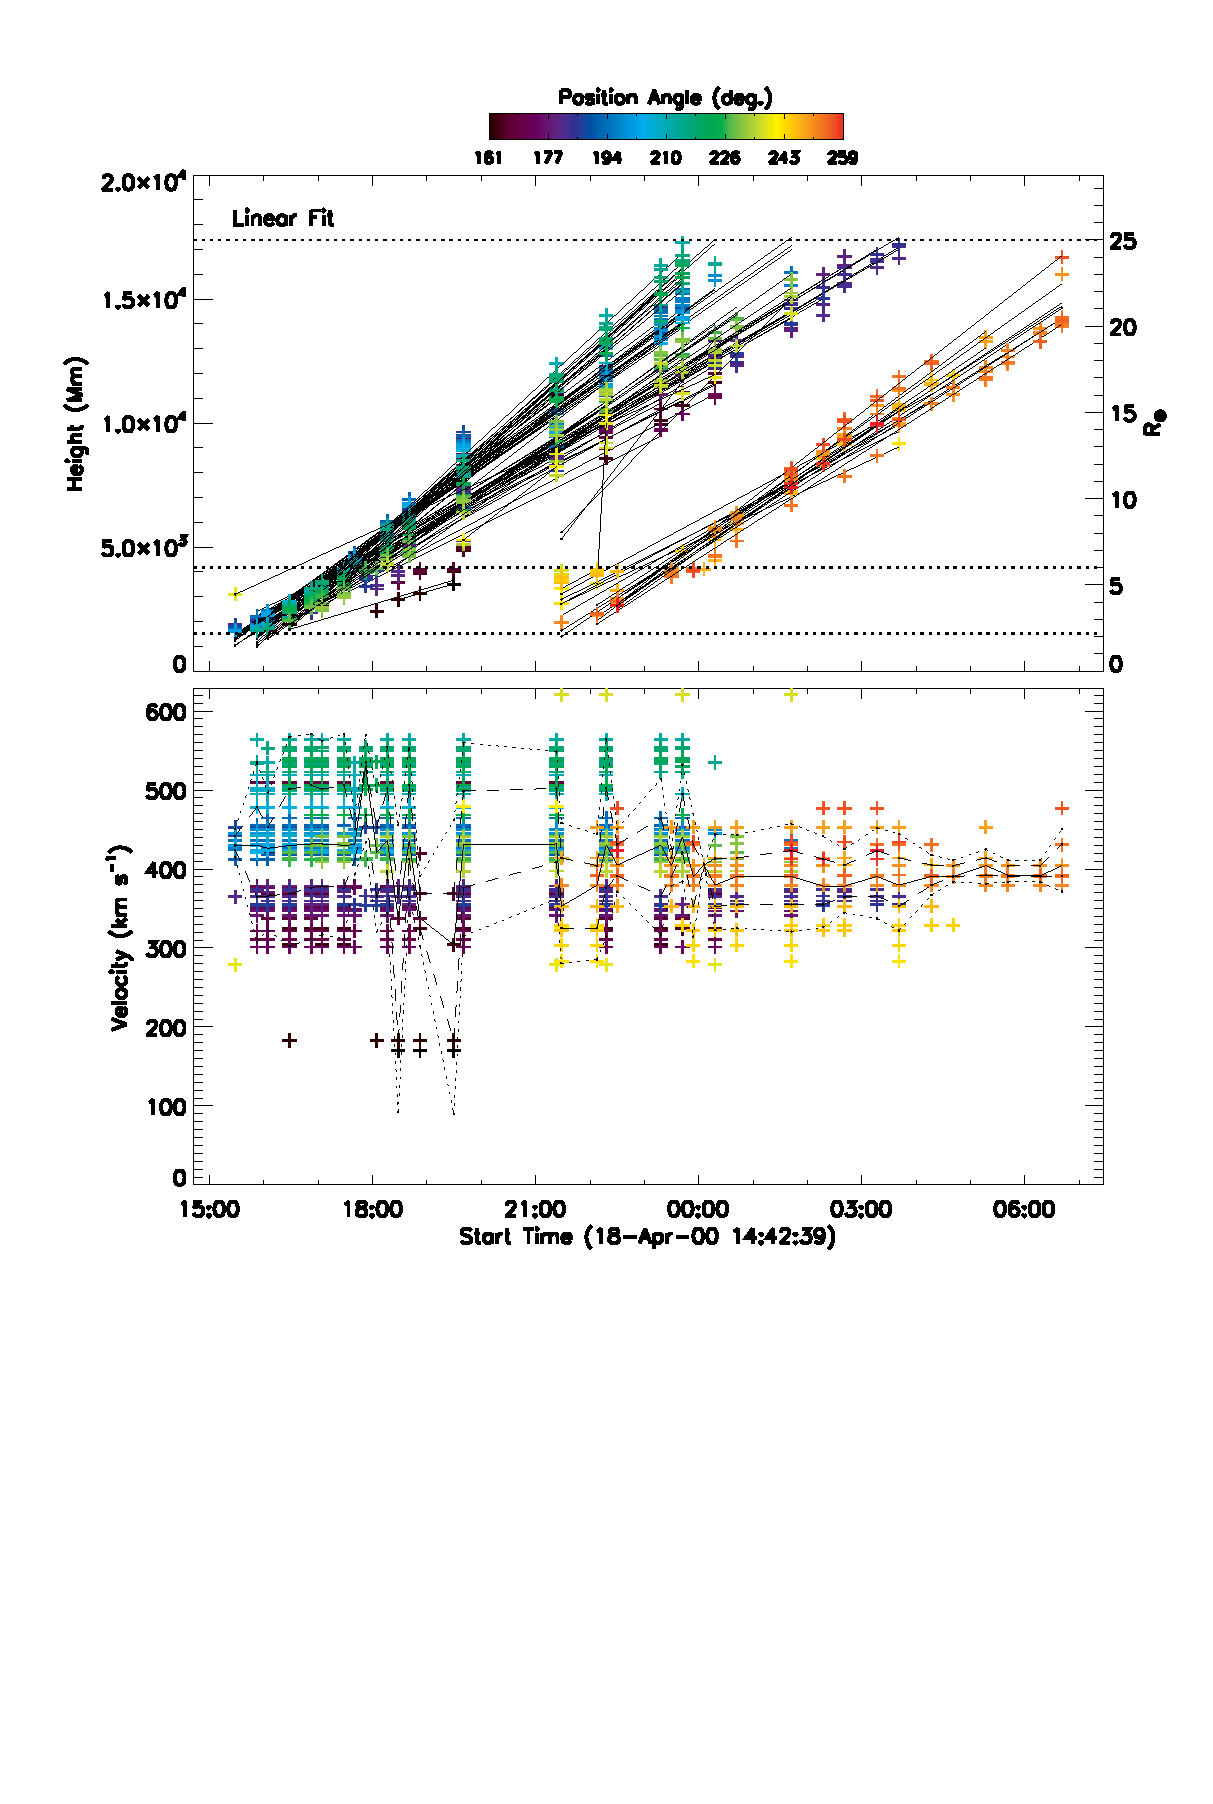
\includegraphics[width=\linewidth]{images/plot_kins_quartiles_linear_20000418_152817.eps}}
\caption{CORIMP linear.}
\label{}
\end{figure}

\begin{figure}[]
\centerline{\includegraphics[width=\linewidth]{images/20000418_cdaw_kins.png}}
\caption{CDAW quadratic.}
\label{}
\end{figure}

\begin{figure}[]
\centerline{\includegraphics[width=\linewidth]{images/20000418_153005_seeds_acc.png}}
\caption{SEEDS quadratic.}
\label{}
\end{figure}

\begin{figure}[]
\centerline{\includegraphics[width=\linewidth]{images/20000418_cactus_speed.png}}
\caption{CACTus linear.}
\label{}
\end{figure}


\begin{table*}
\begin{tabular}{l*{4}{c}r}
\multicolumn{5}{c}{Comparison for LASCO CME on 2000\,Apr.\,18 from $\sim$15:00\,UT} \\
\hline
Catalog              & CPA [deg.] & AW [deg.] & Linear Speed [$km\,s^{-1}$] & Accel. [$m\,s^{-2}$]  \\
\hline
CDAW & 195 & 105 & 668 & 23.1    \\
CORIMP            & 210 & 98 & 431 & 19   \\
CACTUS           & 198 & 102 & 463 & --    \\
SEEDS     & 195 & 108 & 338 & 17.7    \\
\end{tabular}
\end{table*}

\acknowledgments

This work is supported by SHINE grant 0962716 and NASA grant NNX08AJ07G to the Institute for Astronomy. %The \emph{SOHO}/LASCO data used here are produced by a consortium of the Naval Research Laboratory (USA), Max-Planck-Institut fuer Aeronomie (Germany), Laboratoire d'Astronomie (France), and the University of Birmingham (UK). SOHO is a project of international cooperation between ESA and NASA. \emph{SDO} data supplied courtesy of the NASA/\emph{SDO} consortia.
The \emph{STEREO}/SECCHI project is an international consortium of the Naval Research Laboratory (USA), Lockheed Martin Solar and Astrophysics Lab (USA), NASA Goddard Space Flight Center (USA), Rutherford Appleton Laboratory (UK), University of Birmingham (UK), Max-Planck-Institut f\"{u}r Sonnen-systemforschung (Germany), Centre Spatial de Liege (Belgium), Institut d'Optique Th\'{e}orique et Appliqu\'{e}e (France), and Institut d'Astrophysique Spatiale (France).
%\appendix

%\section{Appendix material}

%For completeness, here is one last equation.
%\begin{equation}
%e = mc^2
%\end{equation}

\bibliographystyle{apj.bst}
\bibliography{references.bib}  


\end{document}